\section{Implementation}
\label{sec:Implementation}

\subsection{Frontend}
% SPA -> Frameworks -> Angular -> Google Material Design -> APIs -> Pics

There are many mature SPA frameworks today, such as Vue.js, ReactJS, Angular.js, Angular2, and so on. Since the author is familiar with Angular2, the frontend part of the project is implemented using Angular2, which comes with almost everything we need, from powerful templates to fast rendering, data management, HTTP services, form handling, and so much more. Moreover, Angular2 provides a UI component library called Angular Material,
which is inspired by Google Material Design. Angular Material components help in constructing attractive, consistent, and functional web pages and web applications while adhering to modern web design principles like browser portability, device independence, and graceful degradation. It helps in creating faster, beautiful, and responsive websites.

In our design, the user must register to log in before he can use the application, so the home page is the login page. Luckily, Angular2 provides multiple routing guards, and the CanActivate interface is a good way for us to implement our own authentication routing. In addition, as we mentioned in Section \ref{sec:Requirements>Non-Functional Requirements} Non-Functional Requirements, every form must be validated by the client side before being submitted to the server side. The Implementation of GUI is listed below:

\begin{enumerate}
  \item The ``Sign Up'' form requires the user to enter a unique and valid email, first name, last name, password, and confirmed password. The user can click the icon on the right of the password input to make his password visible or invisible. Also, the ``clear'' button on the left bottom corner is used to clear all inputs of the Sign-Up form. The user can also click the ``Log in instead'' button to be redirected to the ``Log In'' page if he already has an account. Figure \ref{fig:GUI signup} is the interface of the ``Sign Up'' page

  \begin{figure}[htbp]
  \centering
  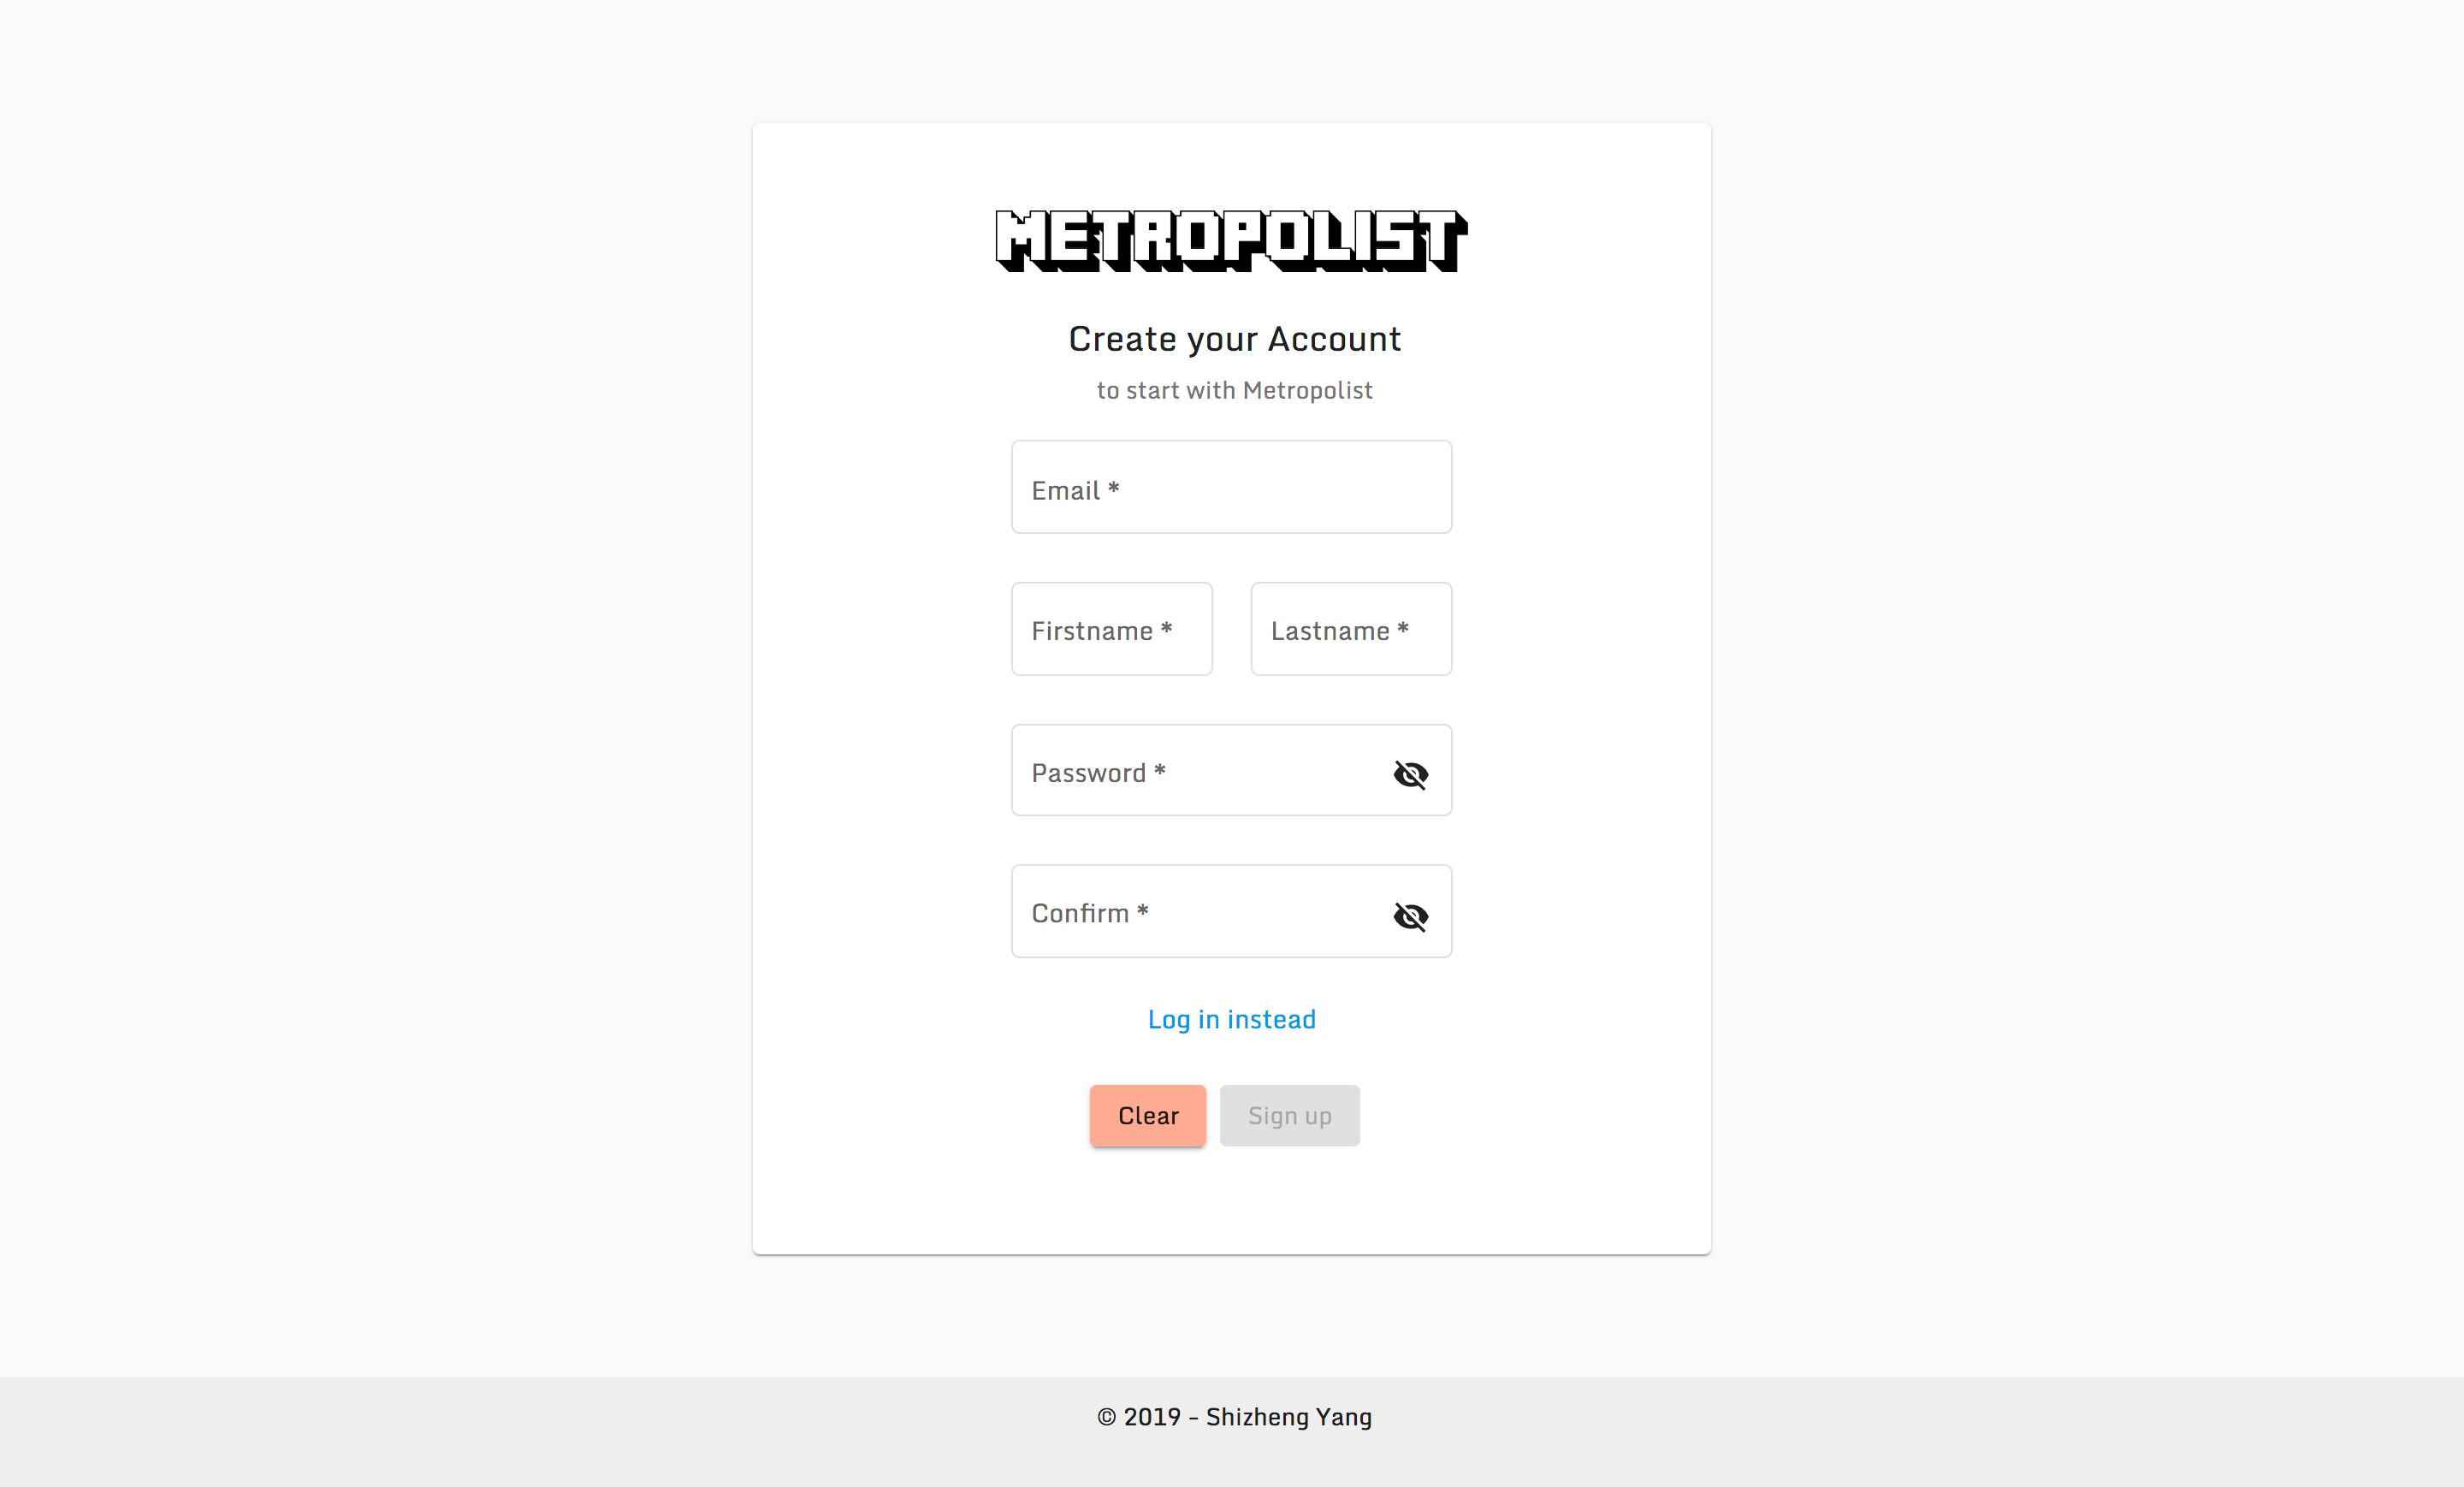
\includegraphics[width=\textwidth]{section04/assets/GUI-signup.png}
  \caption[GUI: Sign Up]{\label{fig:GUI signup}GUI: Sign Up}
  \end{figure}

  \item The ``Log In'' form requires the user to enter the email and the password. Also, the user can access to the Sign-Up page via the ``Create account'' button on the bottom. Figure \ref{fig:GUI login} is the interface of the ``Log In'' page

  \begin{figure}[htbp]
  \centering
  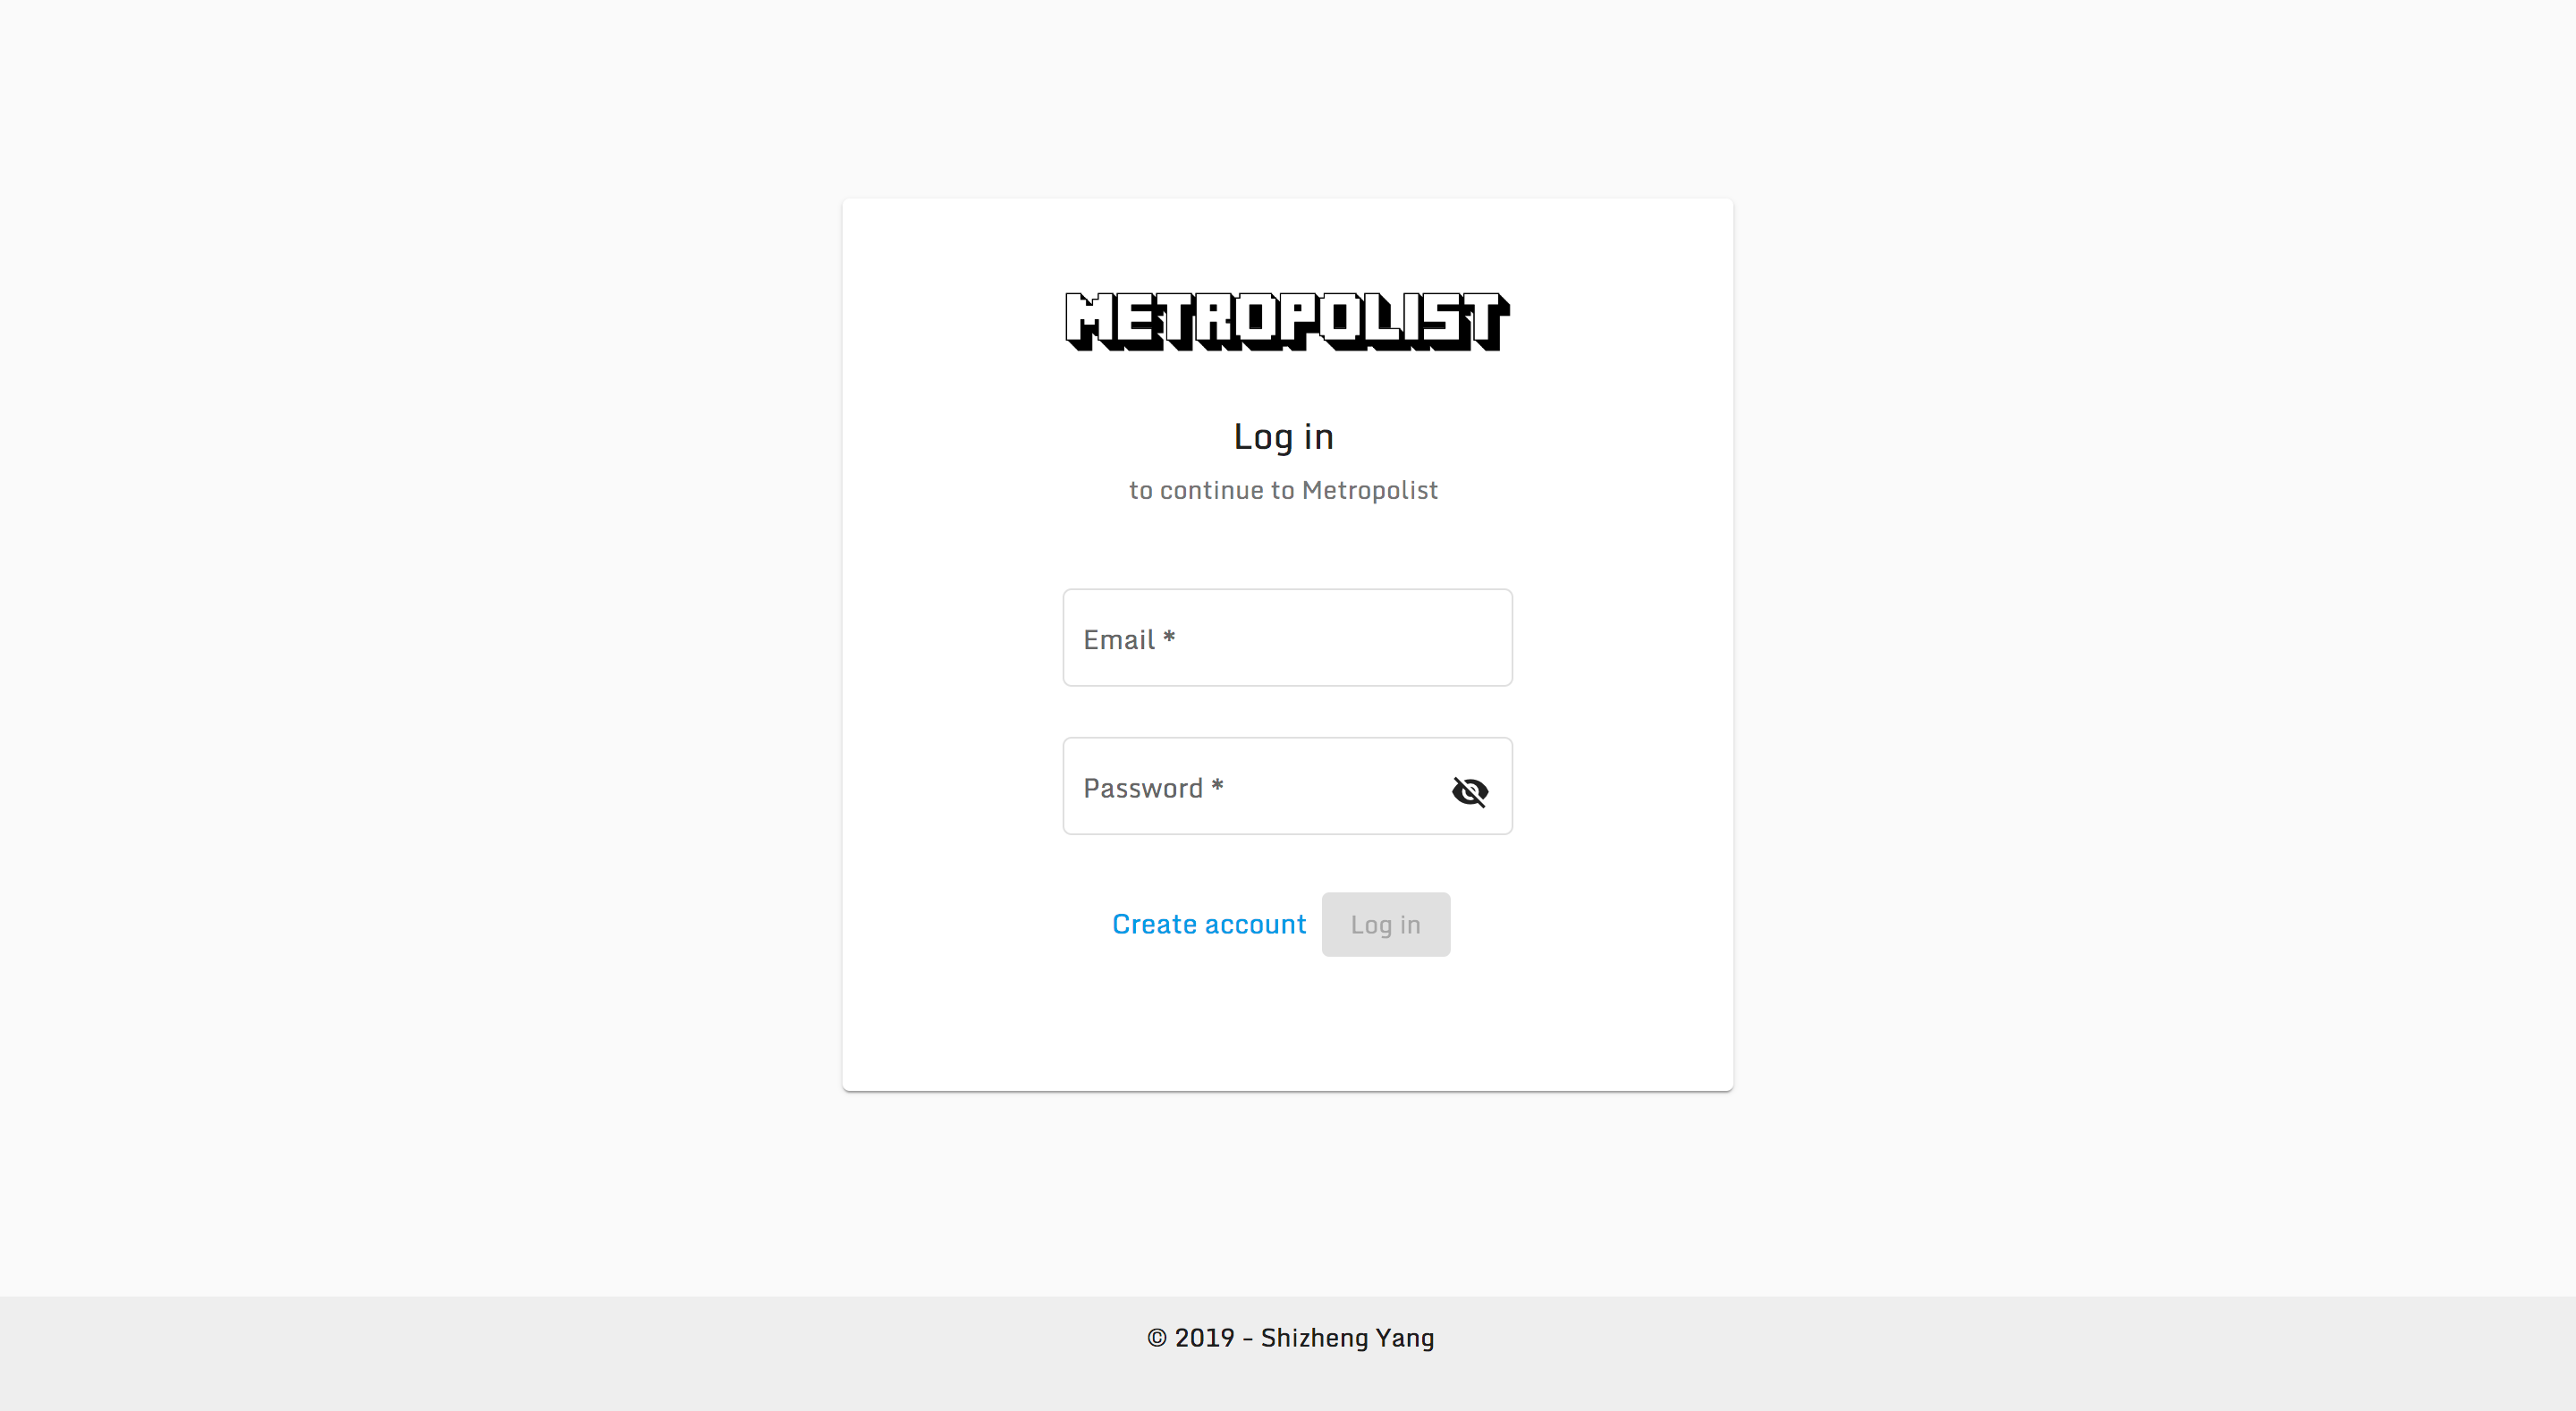
\includegraphics[width=\textwidth]{section04/assets/GUI-login.png}
  \caption[GUI: Log In]{\label{fig:GUI login}GUI: Log In}
  \end{figure}

  \item The ``Community'' page shows all the maps that can be viewed, which are marked by their own owners as ``isVisible.'' Besides, the user can filter maps using map name, owner's email, owner's first name, or owner's last name via the ``Filter'' input on the left top corner. Figure \ref{fig:GUI community} is the interface of the ``Community'' page

  \begin{figure}[htbp]
  \centering
  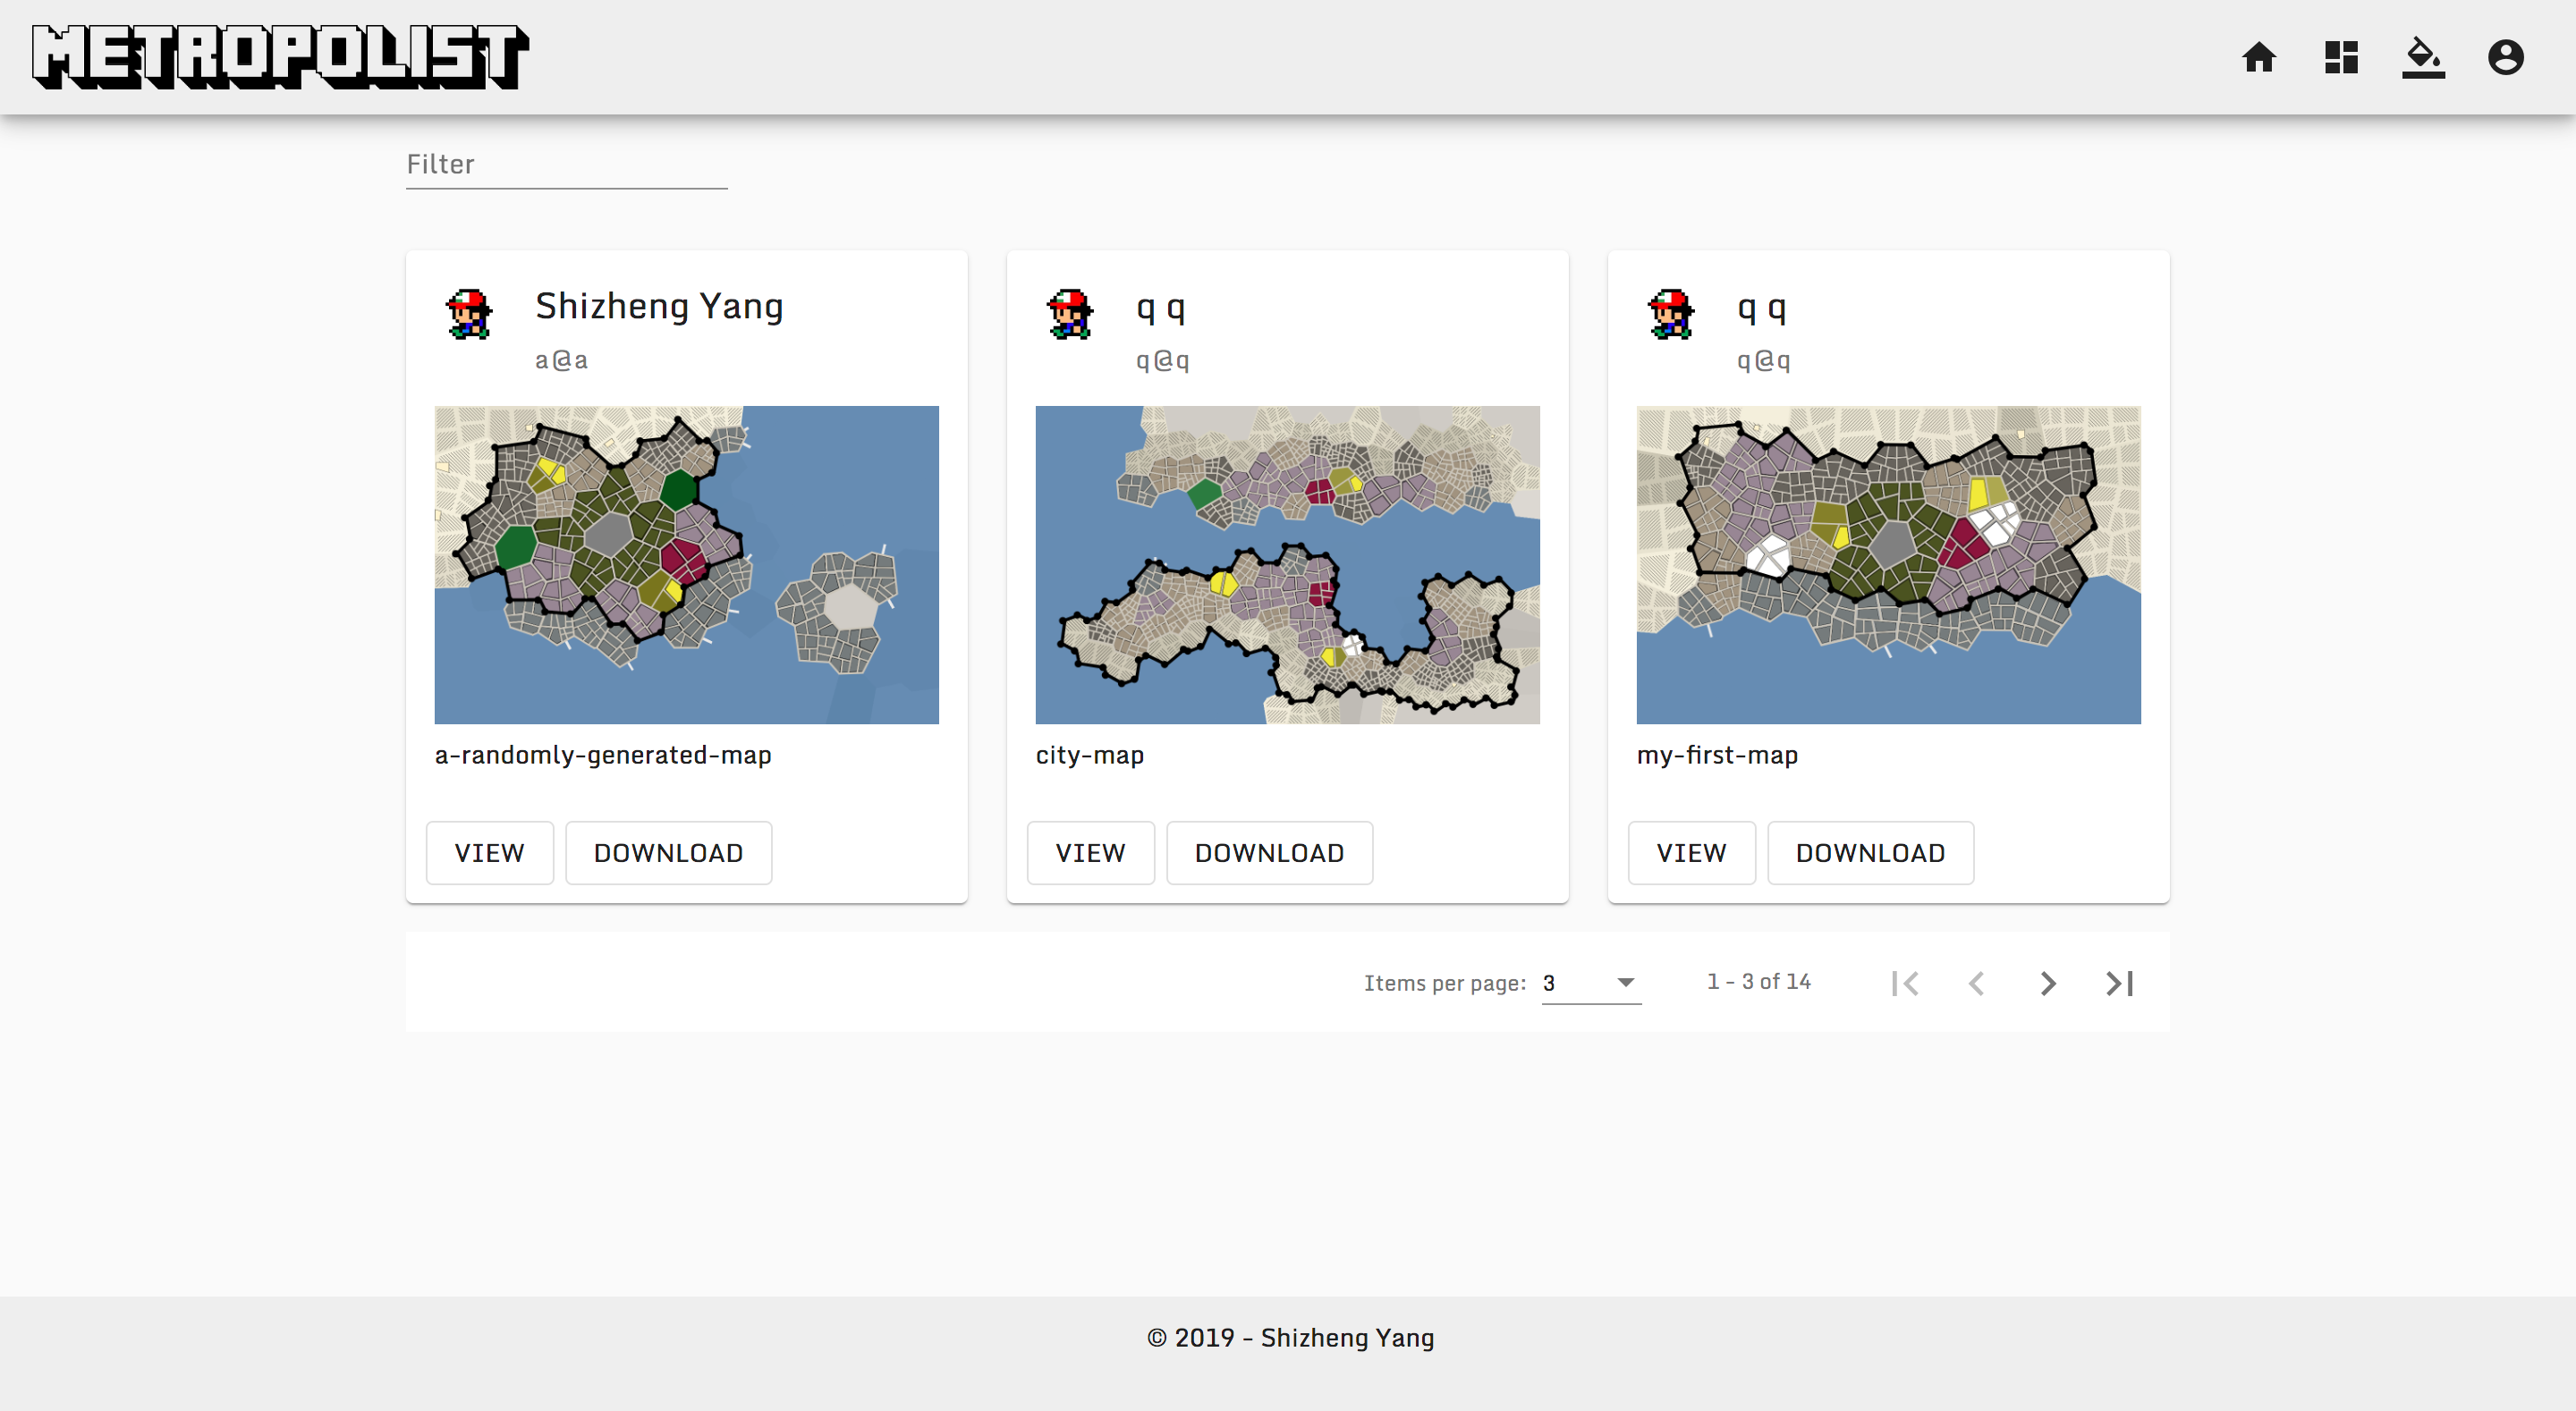
\includegraphics[width=\textwidth]{section04/assets/GUI-community.png}
  \caption[GUI: Community]{\label{fig:GUI community}GUI: Community}
  \end{figure}

  \item The ``User Dashboard'' page displays all the maps belong to the current user. The user can filter them using any information of maps via the ``Filter'' input on the left top corner. The user can click on the header to perform the sorting of the corresponding map properties. Also, the user is allowed to make the map be visible or invisible by manipulating the slide of ``isVisible'', and edit, delete or download it via the three buttons in the ``Operation'' column. In addition, The button for creating a new map is in the lower right corner of the page, the user can enter a map name in the pop-up window after clicking it. Figure \ref{fig:GUI user dashboard} is the interface of the User dashboard page

  \begin{figure}[htbp]
  \centering
  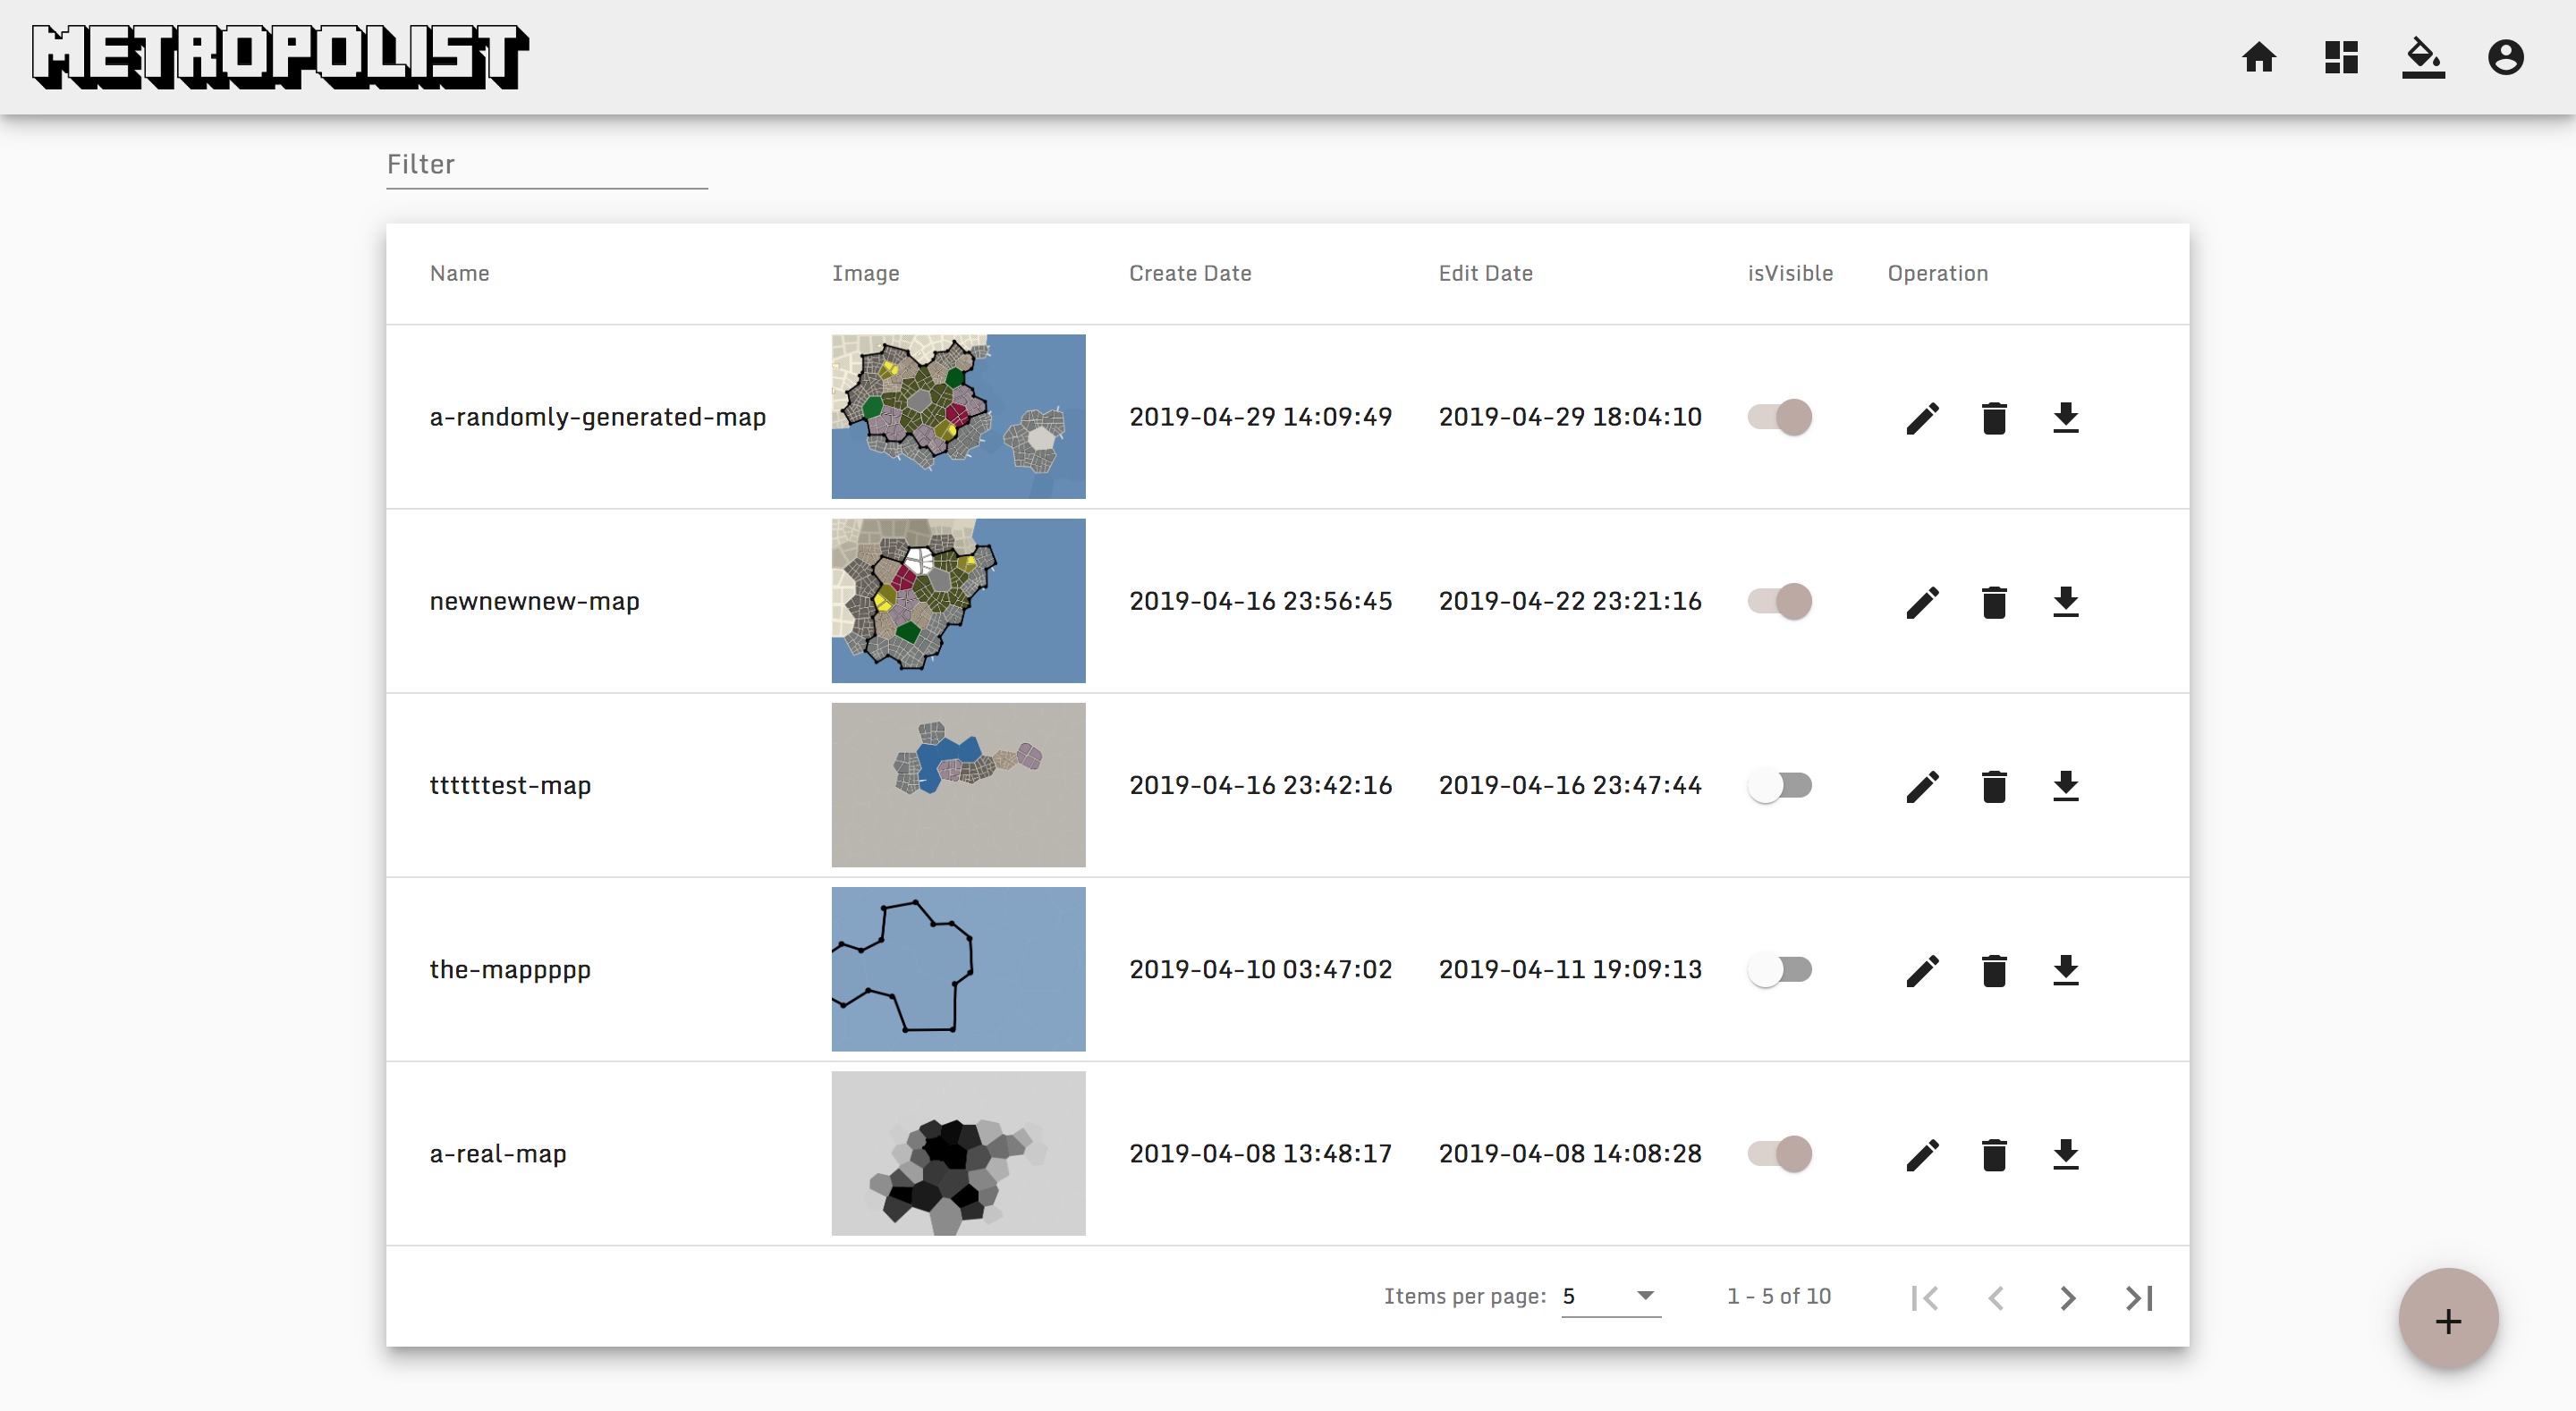
\includegraphics[width=\textwidth]{section04/assets/GUI-user.png}
  \caption[GUI: User Dashboard]{\label{fig:GUI user dashboard}GUI: User Dashboard}
  \end{figure}

  \item The ``Profile'' page allows the user to change his email, password, or names. By the way, before changing the password, the user must first enter the old password. After the verification is passed, the new password can be entered. Figure \ref{fig:GUI profile} is the interface of the Profile page

  \begin{figure}[htbp]
  \centering
  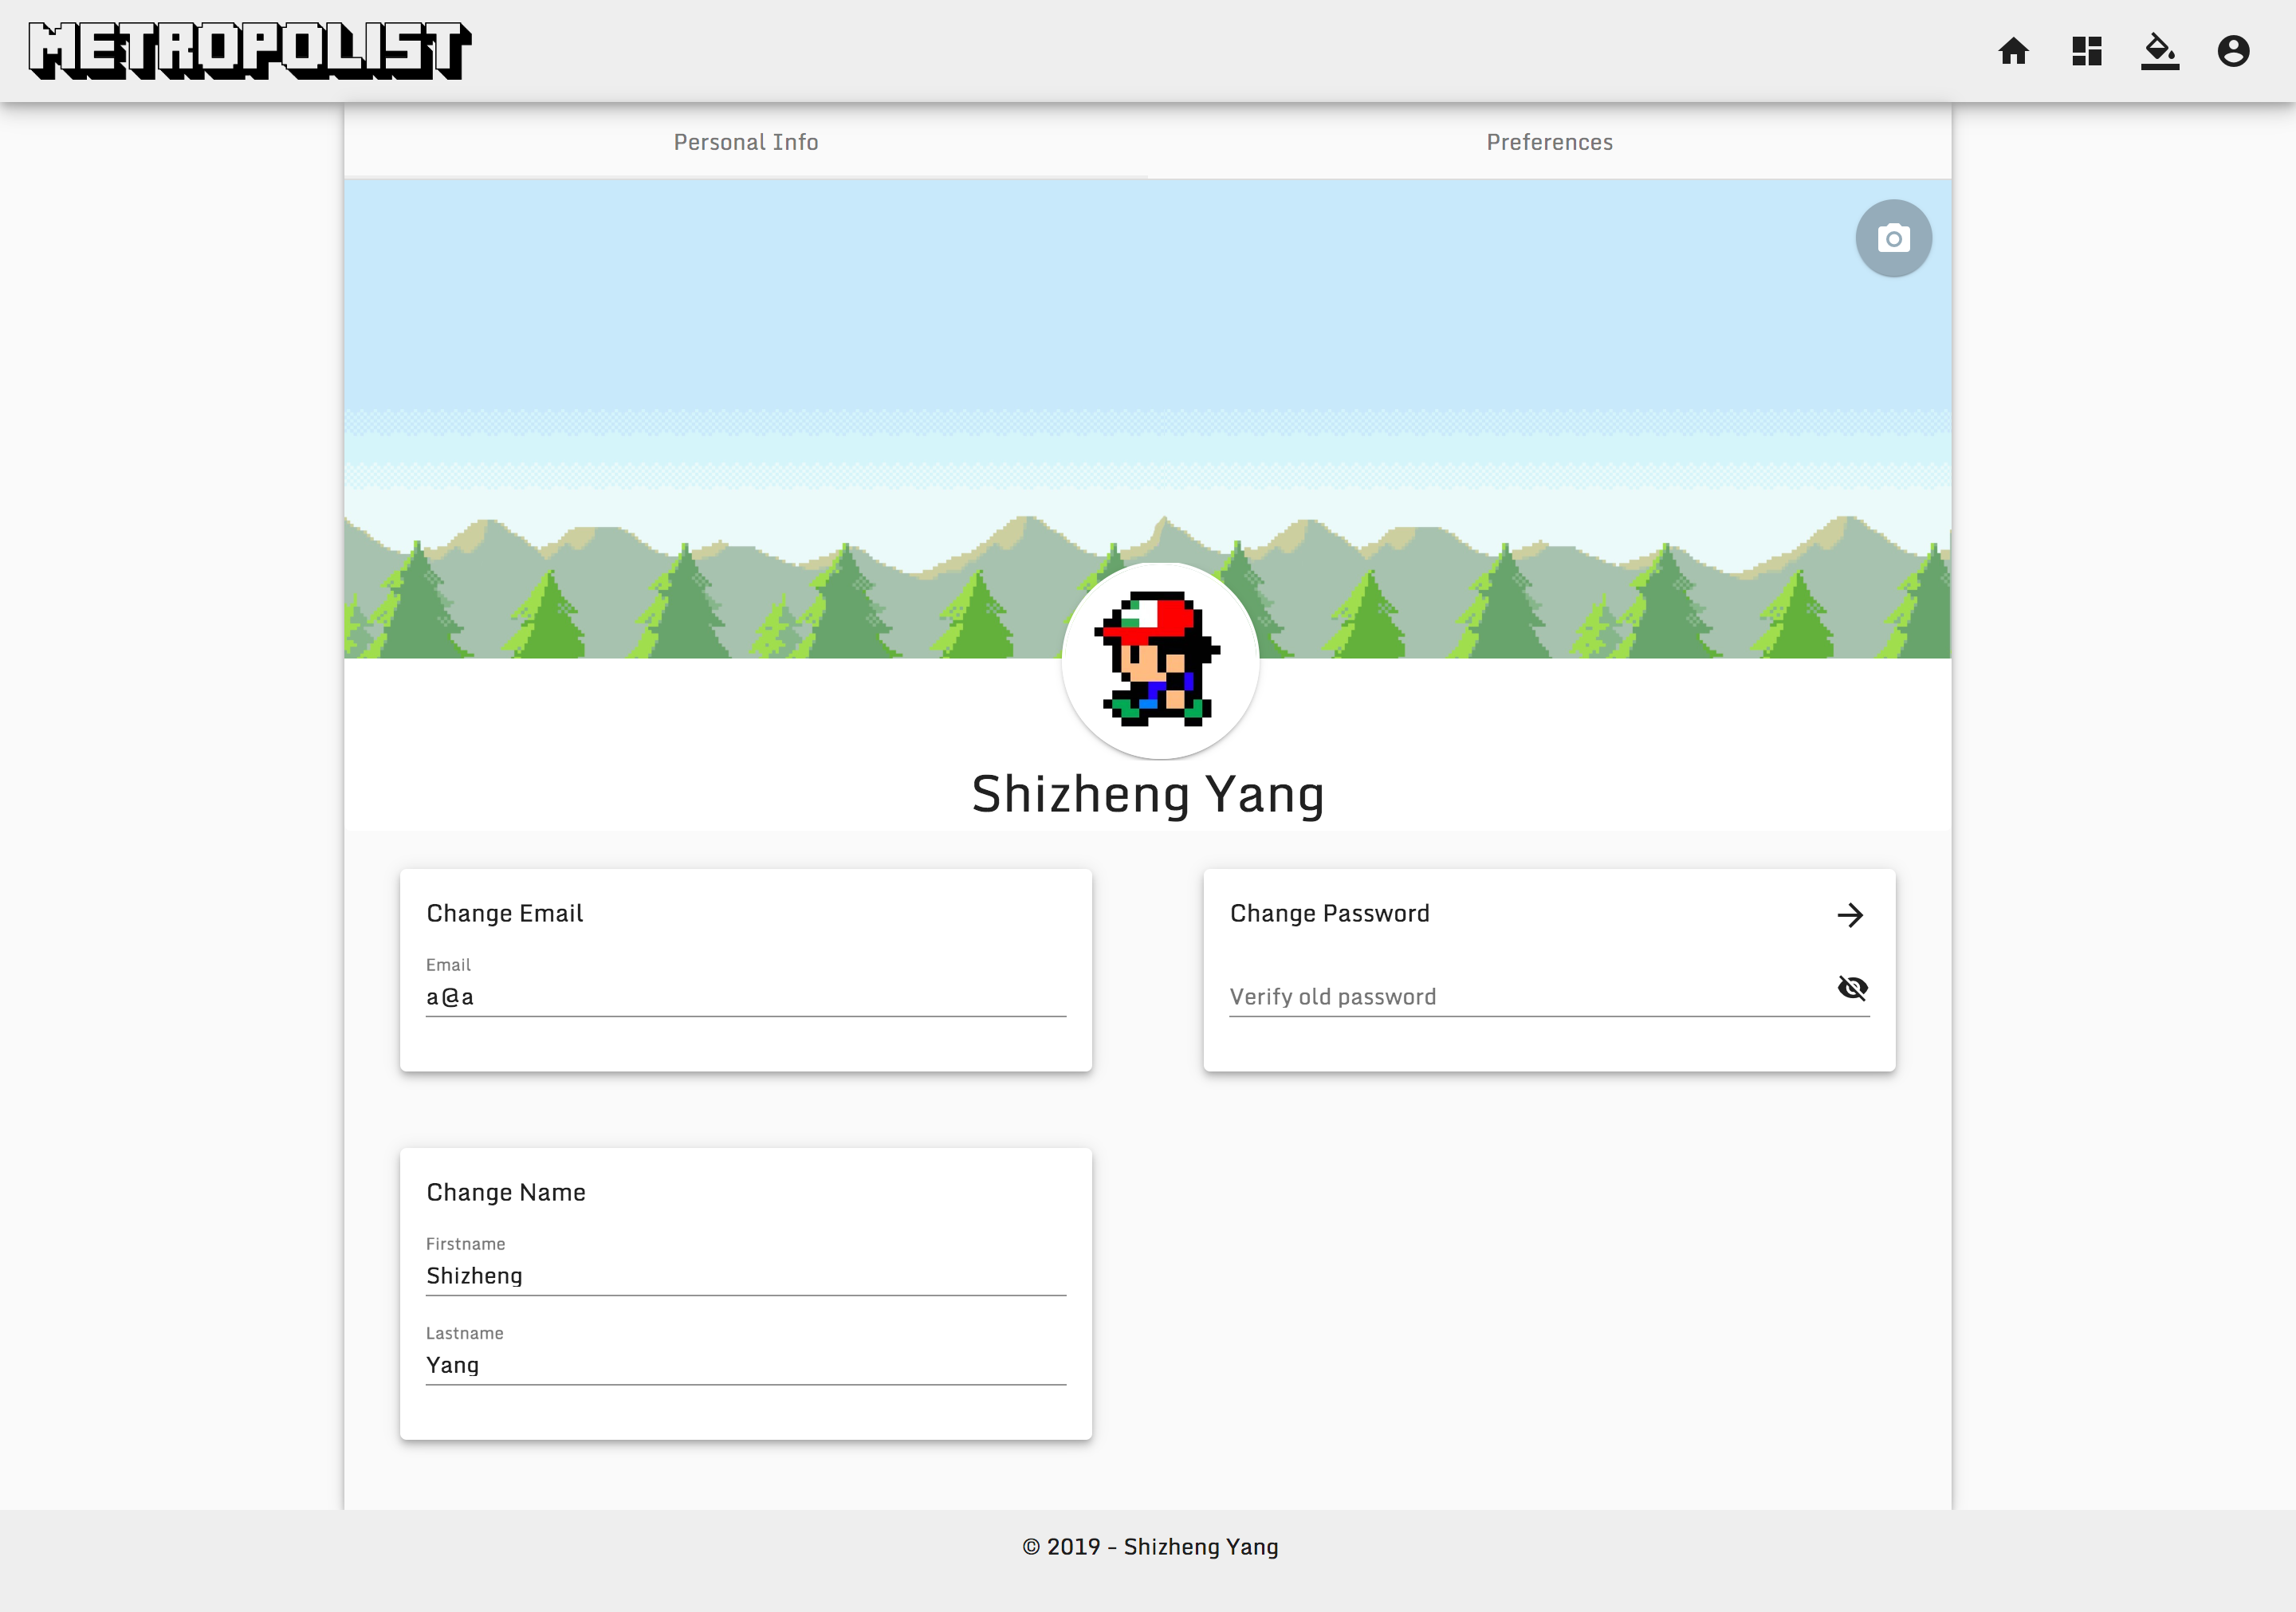
\includegraphics[width=\textwidth]{section04/assets/GUI-profile.png}
  \caption[GUI: Profile]{\label{fig:GUI profile}GUI: Profile}
  \end{figure}

\end{enumerate}

\subsection{Backend}
% Node.js Express -> Auth -> REST APIs -> MongoDB

\subsection{Map Generator}
% Voronoi -> Lloyd's Relaxation -> D3 mouse events -> Layers: elevation, affluence,
